% Module 2: How Claude Code Works
% Beamer Presentation — Claude Code for Academic Researchers
\documentclass[aspectratio=169, 11pt]{beamer}

% ── Theme and Colors ──────────────────────────────────────────────
\usetheme{Madrid}
\usecolortheme{default}

% Custom colors
\definecolor{anthropic}{RGB}{50, 50, 80}
\definecolor{accent}{RGB}{180, 90, 40}
\definecolor{lightgray}{RGB}{245, 245, 245}

\setbeamercolor{structure}{fg=anthropic}
\setbeamercolor{frametitle}{bg=anthropic, fg=white}
\setbeamercolor{title}{bg=anthropic, fg=white}
\setbeamercolor{block title}{bg=anthropic, fg=white}
\setbeamercolor{block body}{bg=lightgray}
\setbeamercolor{alerted text}{fg=accent}

\setbeamerfont{title}{size=\Large, series=\bfseries}
\setbeamerfont{frametitle}{size=\large, series=\bfseries}

% ── Packages ──────────────────────────────────────────────────────
\usepackage{graphicx}
\usepackage{booktabs}
\usepackage{listings}
\usepackage{fontenc}
\usepackage{hyperref}
\usepackage{tikz}

\lstset{
  basicstyle=\ttfamily\small,
  backgroundcolor=\color{lightgray},
  frame=single,
  framerule=0pt,
  breaklines=true,
  columns=fullflexible,
}

% ── Metadata ──────────────────────────────────────────────────────
\title{Module 2: How Claude Code Works}
\subtitle{Claude Code for Academic Researchers}
\author{} % Instructor name
\date{}
\institute{}

% ══════════════════════════════════════════════════════════════════
\begin{document}

% ── Title ─────────────────────────────────────────────────────────
\begin{frame}[plain]
  \titlepage
\end{frame}

% ══════════════════════════════════════════════════════════════════
%  FROM INTERACTIVE TO FILE-BASED  [0:00–8:00]
% ══════════════════════════════════════════════════════════════════

\begin{frame}{From Interactive to File-Based Workflows}
  \textbf{What you do now} (Stata / R):
  \begin{itemize}
    \item Open a session, load data into memory
    \item Run commands interactively, see results immediately
  \end{itemize}

  \vspace{0.8em}
  \textbf{How Claude Code works}:
  \begin{itemize}
    \item Reads and writes \textbf{files on disk}
    \item No persistent session with your data loaded
    \item Reads your files $\rightarrow$ writes/modifies scripts $\rightarrow$ optionally runs them
  \end{itemize}
\end{frame}

\begin{frame}{Practical Implication}
  \begin{alertblock}{Think in Projects, Not Sessions}
    You need to think in terms of:
    \begin{itemize}
      \item Project directories
      \item File paths
      \item Scripts that run end-to-end
    \end{itemize}
    Not interactive exploration.
  \end{alertblock}
\end{frame}

% ══════════════════════════════════════════════════════════════════
%  THE CONTEXT WINDOW  [8:00–12:00]
% ══════════════════════════════════════════════════════════════════

\begin{frame}{The Context Window}
  Claude Code can only ``see'' a limited amount of text at once.

  \vspace{0.5em}
  The context window includes:
  \begin{itemize}
    \item Your instructions
    \item The files it reads
    \item Its own responses
  \end{itemize}

  \vspace{0.8em}
  \alert{When a conversation gets long or a project gets large, it loses earlier context.}
\end{frame}

\begin{frame}{Why the Context Window Matters}
  \begin{block}{The Consistency Problem}
    In a complex project with many files, Claude Code may change one file in a way that is \textbf{inconsistent} with another file it can no longer see.
  \end{block}

  \vspace{0.5em}
  \textbf{Strategies:}
  \begin{itemize}
    \item Keep tasks focused
    \item Provide only relevant context
    \item Tell Claude Code explicitly which files matter
  \end{itemize}
\end{frame}

% ══════════════════════════════════════════════════════════════════
%  THE THREE EXECUTION MODES  [12:00–30:00]
% ══════════════════════════════════════════════════════════════════

\begin{frame}{The Three Execution Modes}
  \centering
  {\large The most important configuration decision you will make.}

  \vspace{1em}
  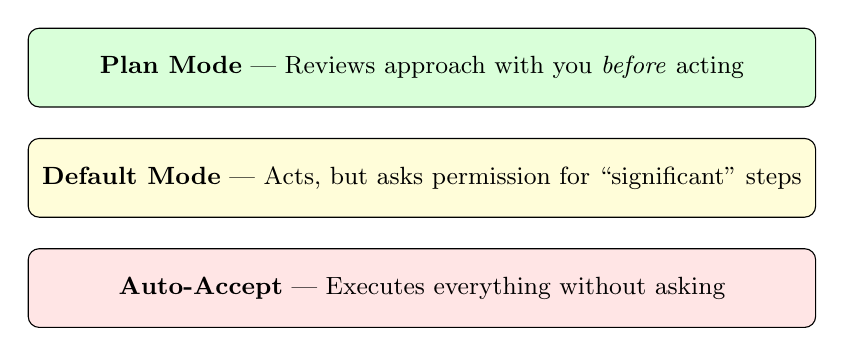
\begin{tikzpicture}[
    node distance=0.4cm,
    every node/.style={draw, rounded corners, minimum width=10cm, minimum height=1cm, align=center, font=\small}
  ]
    \node[fill=green!15] (plan) at (0,2.8) {\textbf{Plan Mode} --- Reviews approach with you \textit{before} acting};
    \node[fill=yellow!15] (default) at (0,1.4) {\textbf{Default Mode} --- Acts, but asks permission for ``significant'' steps};
    \node[fill=red!10] (auto) at (0,0) {\textbf{Auto-Accept} --- Executes everything without asking};
  \end{tikzpicture}

  \vspace{0.5em}
  \small $\downarrow$ More autonomy, less oversight $\downarrow$
\end{frame}

\begin{frame}{Plan Mode \hfill \normalsize\textit{Recommended Default for Research}}
  \textbf{How it works:}
  \begin{itemize}
    \item Claude Code analyzes your request
    \item Proposes a detailed plan (files to read, changes to make, approach)
    \item Waits for your explicit approval before acting
    \item You review, approve, modify, or reject
  \end{itemize}

  \vspace{0.5em}
  \textbf{When to use:}\\
  Any task where the \textit{approach} matters, not just the output.\\
  Data transformation, variable construction, merges, anything analytical.

  \vspace{0.5em}
  \begin{block}{Why It Matters}
    The plan is your checkpoint. This is where you catch ``I am going to do an inner join'' \textit{before} it happens---not after 300 observations are gone.
  \end{block}
\end{frame}

\begin{frame}{Default Mode \hfill \normalsize\textit{Use With Caution}}
  \textbf{How it works:}
  \begin{itemize}
    \item Claude Code executes steps autonomously
    \item Pauses for actions \textit{it} considers significant
    \item Uses its own judgment about when to ask
  \end{itemize}

  \vspace{0.5em}
  \textbf{When to use:}\\
  Routine tasks in established projects where you trust the general approach.

  \vspace{0.8em}
  \begin{alertblock}{The Risk for Academics}
    Claude Code's judgment about what is ``significant'' may not match yours.\\
    It might pause before writing a file but \textbf{not} before silently recoding a variable.
  \end{alertblock}
\end{frame}

\begin{frame}{Auto-Accept Mode \hfill \normalsize\textit{Low-Risk Tasks Only}}
  \textbf{How it works:}
  \begin{itemize}
    \item Executes everything without asking
    \item Reads, writes, runs, and modifies freely
    \item Stops only on errors
  \end{itemize}

  \vspace{0.5em}
  \textbf{When to use:}
  \begin{itemize}
    \item File reformatting
    \item Boilerplate generation
    \item Documentation
  \end{itemize}

  \vspace{0.5em}
  \textbf{When \alert{not} to use:}\\
  Anything involving your data or analysis.\\
  The speed gain is not worth the loss of checkpoints.
\end{frame}

\begin{frame}{The Key Insight on Modes}
  \begin{alertblock}{Different Relationships with the Agent}
    \textbf{Plan mode} = you \textbf{direct} the work\\
    \textbf{Auto-accept} = you \textbf{review} the work after the fact
  \end{alertblock}

  \vspace{0.8em}
  For published research, directing is almost always safer than reviewing after the fact.

  \vspace{0.5em}
  \textbf{Why:} Errors you \textit{prevent} at the planning stage are cheaper than errors you \textit{catch} in the output---or worse, errors you don't catch at all.
\end{frame}

% ══════════════════════════════════════════════════════════════════
%  LIVE DEMO: PLAN vs AUTO-ACCEPT
% ══════════════════════════════════════════════════════════════════

\begin{frame}{Live Demo: Plan Mode vs. Auto-Accept}
  \centering
  \vfill
  Same task, two modes.

  \vspace{0.5em}
  Watch for:
  \begin{itemize}
    \item What does a plan look like?
    \item How do you evaluate it?
    \item What does the experience feel like in each mode?
  \end{itemize}
  \vfill
  {\footnotesize\textit{[Switch to terminal]}}
\end{frame}

% ══════════════════════════════════════════════════════════════════
%  CLAUDE.MD  [30:00–40:00]
% ══════════════════════════════════════════════════════════════════

\begin{frame}{CLAUDE.md: Your Lab Notebook for the Agent}
  A file in your project directory that Claude Code reads \textbf{automatically}.

  \vspace{0.5em}
  It encodes your conventions, definitions, and constraints.

  \vspace{0.5em}
  \textbf{The single most effective way to prevent errors before they happen.}
\end{frame}

\begin{frame}{What Belongs in CLAUDE.md}
  \begin{columns}[T]
    \begin{column}{0.48\textwidth}
      \textbf{Include:}
      \begin{itemize}
        \item Project description \& research question
        \item Data structure: files, key variables, units, expected ranges
        \item Coding conventions
      \end{itemize}
    \end{column}
    \begin{column}{0.48\textwidth}
      \textbf{Include (cont.):}
      \begin{itemize}
        \item Constraints: ``never drop observations without logging''
        \item ``All merges must report row counts''
        \item What Claude Code should \textbf{not} do
      \end{itemize}
    \end{column}
  \end{columns}
\end{frame}

\begin{frame}[fragile]{CLAUDE.md Example}
\begin{lstlisting}
# CLAUDE.md - County Migration Project

## Research Question
Effect of historical migration on county-level outcomes.

## Data
- data/raw/census_panel.csv: county-year panel, 1920-2020
- Key vars: fips (5-digit), year, population, migration_share
- All monetary values in 2020 USD

## Constraints
- Never drop observations without logging count and reason
- All merges must report pre- and post-merge row counts
- Always use robust standard errors
- Do not choose model specifications
- Do not interpret coefficients
\end{lstlisting}
\end{frame}

% ══════════════════════════════════════════════════════════════════
%  COST MANAGEMENT  [40:00–48:00]
% ══════════════════════════════════════════════════════════════════

\begin{frame}{Cost Management}
  \begin{alertblock}{A Real Constraint}
    On the \$20/month plan, you can burn through your allocation in 30--45 minutes of active use if you are not strategic.
  \end{alertblock}

  \vspace{0.5em}
  \textbf{Principles:}
  \begin{enumerate}
    \item Not everything needs Claude Code---small edits are faster by hand
    \item A well-written CLAUDE.md reduces back-and-forth (= fewer tokens)
    \item If Claude Code is spinning on a wrong approach, \textbf{intervene early}
    \item Batch related tasks into one well-scoped request
    \item Plan mode adds tokens but prevents costly wrong approaches
  \end{enumerate}
\end{frame}

% ══════════════════════════════════════════════════════════════════
%  EXERCISE  [48:00–70:00]
% ══════════════════════════════════════════════════════════════════

\begin{frame}{Exercise: Set Up a Project in Plan Mode}
  Work in pairs:
  \begin{enumerate}
    \item Create a project directory:
      \begin{itemize}
        \item \texttt{data/}, \texttt{scripts/}, \texttt{output/}
      \end{itemize}
    \item Write a \texttt{CLAUDE.md} from the template\\
      {\small (for the provided scenario or your own project)}
    \item Switch Claude Code to plan mode
    \item Issue a task:\\
      {\small ``Write a script that loads \texttt{data/raw/survey.csv} and prints summary statistics''}
    \item \textbf{Review the plan} before approving
    \item Approve $\rightarrow$ run $\rightarrow$ verify the output
  \end{enumerate}
\end{frame}

\begin{frame}{Evaluating a Plan}
  When you see Claude Code's plan, ask:
  \begin{itemize}
    \item Does it match what I intended?
    \item Is it reading the right files?
    \item What join type / transformation is it proposing?
    \item Would I change anything before approving?
  \end{itemize}

  \vspace{0.8em}
  \alert{Plans are not rubber stamps.}\\
  If the plan includes a questionable choice, \textbf{reject or modify it}.
\end{frame}

% ══════════════════════════════════════════════════════════════════
%  DEBRIEF  [70:00–75:00]
% ══════════════════════════════════════════════════════════════════

\begin{frame}{Debrief}
  \begin{itemize}
    \item What did you put in your CLAUDE.md?
    \item What did the plan look like---was it what you expected?
    \item Did anyone reject or modify a plan?
  \end{itemize}

  \vspace{0.8em}
  \begin{block}{Two Habits That Pay Off}
    \textbf{Writing a CLAUDE.md} forces you to be explicit about conventions you have kept implicit.

    \vspace{0.3em}
    \textbf{Reviewing plans} forces you to think about approach \textit{before} you see output.
  \end{block}
\end{frame}

% ══════════════════════════════════════════════════════════════════
%  SUMMARY
% ══════════════════════════════════════════════════════════════════

\begin{frame}{Module 2 Summary}
  \begin{enumerate}
    \item Claude Code works with \textbf{files}, not interactive sessions
    \item The \textbf{context window} limits what it can hold---keep tasks focused
    \item \textbf{Plan mode} is the default for research work
    \item \textbf{CLAUDE.md} is your most powerful tool for preventing errors
    \item \textbf{Cost management} is a core skill, not an afterthought
  \end{enumerate}

  \vspace{1em}
  \centering
  \textbf{Next: Module 3 --- Automating Research Tasks}
\end{frame}

\end{document}
